% MHIPEX: Multilingual Historical Person-Place Relation Extraction
% CLEF 2026 Working Notes — LNCS Format
\documentclass[runningheads]{llncs}
\usepackage[T1]{fontenc}
\usepackage{graphicx}
\usepackage{booktabs}
\usepackage{multirow}
\usepackage{amsmath}
\usepackage{hyperref}
\usepackage{xcolor}

\begin{document}

\title{MHIPEX: An Enriched Transformer Ensemble for\\Person--Place Relation Extraction from\\Multilingual Historical Newspapers}

\author{Aman Jaiswal \and Sarika Jain}
\authorrunning{Jaiswal and Jain}
\institute{National Institute of Technology Kurukshetra, India}

\maketitle

\begin{abstract}
This paper presents MHIPEX, a knowledge-aware system for person--place relation extraction from multilingual historical newspapers, developed in the context of the CLEF HIPE-2026 shared task. MHIPEX combines two complementary transformer encoders---a historically pre-trained multilingual BERT (hmBERT) and XLM-RoBERTa---into a weighted soft-voting ensemble, augmented with enriched input representations (publication date and source language tokens), multi-sample dropout with dual pooling, class-weighted training, and post-hoc threshold calibration. A novel Knowledge Graph augmentation experiment, injecting Wikidata biographical and geographic facts directly into the model's context, reveals a fundamental dichotomy: static KG facts improve spatial relation extraction (\texttt{at} recall +1.6 percentage points) but degrade temporal event extraction (\texttt{isAt} recall $-$1.6\,pp), exposing the need for timeline-aware reasoning beyond static fact retrieval. On the HIPE-2026 sandbox development data, MHIPEX achieves a macro-recall of 0.5655, a +32.5\% relative improvement over a vanilla mBERT baseline. Cross-dataset validation on the separate newspaper v1.0 collection yields an MR of 0.588, confirming domain generalization.
\end{abstract}

\keywords{Historical NLP \and Relation Extraction \and Multilingual Transformers \and Knowledge Graphs \and CLEF HIPE-2026}

%================================================================
\section{Introduction}
\label{sec:intro}
%================================================================

Historical newspapers constitute one of the richest documentary sources for studying population movement, social networks, and geographical ties across centuries. Millions of pages have been digitized in recent decades, yet extracting structured knowledge from them remains a formidable challenge. Optical character recognition (OCR) introduces noise at the character level; archaic orthography and morphology differ substantially from the modern text on which most language models are pre-trained; and the sheer linguistic diversity of European newspaper archives demands systems that can operate across multiple languages simultaneously.

The CLEF HIPE evaluation campaigns have driven sustained progress on information extraction from these sources. The inaugural HIPE-2020 edition~\cite{ehrmann2020} and its successor HIPE-2022~\cite{ehrmann2022} focused on named entity recognition and linking. HIPE-2026~\cite{opitz2026} marks a significant departure: rather than identifying \emph{which} entities appear in a document, participants must now determine the \emph{nature of the relationship} between a person and a place. Concretely, given a (person, location) pair and the newspaper article in which both are mentioned, the system must classify two relations:
\begin{itemize}
    \item \textbf{\texttt{at}}: Did this person ever reside at, travel to, or otherwise have a geographical connection to this place? (three-way: \textsc{false}, \textsc{probable}, \textsc{true})
    \item \textbf{\texttt{isAt}}: Is this person located at this place around the time the article was published? (binary: \textsc{false}, \textsc{true})
\end{itemize}

This formulation poses difficulties that go well beyond standard relation classification. The \texttt{at} relation requires world knowledge---a person may have been born in a city mentioned only in passing---while \texttt{isAt} demands temporal reasoning grounded in the publication date. Both relations exhibit severe class imbalance: in the development data, only 12.0\% of pairs carry a \textsc{true} label for \texttt{at}, and a mere 8.4\% for \texttt{isAt}.

In this work we present MHIPEX (\textbf{M}ultilingual \textbf{H}istorical \textbf{I}nformation \textbf{P}erson-place \textbf{EX}traction), our participating system. We pursue four research questions:

\begin{description}
    \item[RQ1] Can multilingual transformer encoders effectively model person--place relations in noisy historical text?
    \item[RQ2] Does enriching the input with explicit date and language tokens improve classification, particularly for the temporally grounded \texttt{isAt} relation?
    \item[RQ3] Does combining historically and generally pre-trained encoders via ensemble learning yield complementary gains?
    \item[RQ4] Which architectural and training choices contribute most to overall performance, and where do the remaining errors concentrate?
\end{description}

Our results show that MHIPEX achieves a macro-recall (MR) of 0.5655 on the development set, a substantial improvement over each individual baseline. Through ablation we find that the ensemble itself provides the single largest gain (+0.013~MR), while input enrichment and threshold calibration each contribute meaningful increments. Error analysis reveals that the three-way \texttt{at} classification---and in particular the \textsc{probable} class---remains the principal bottleneck.

%================================================================
\section{Related Work}
\label{sec:related}
%================================================================

\subsection{Information Extraction from Historical Documents}

The computational analysis of historical text has gained momentum over the past decade, driven by large-scale digitization projects such as Impresso~\cite{romanello2020} and Europeana Newspapers. Early work focused on adapting NER systems to the unique challenges of historical language. Labusch et al.~\cite{labusch2019} demonstrated that BERT-based models could be successfully applied to German historical texts despite significant orthographic variation, achieving F1 scores above 0.80 on manually annotated corpora.

The HIPE shared task series formalized this line of research into a competitive benchmark. HIPE-2020~\cite{ehrmann2020} attracted 13 teams and established that transformer-based systems consistently outperformed BiLSTM architectures on historical NER, provided sufficient training data was available. HIPE-2022~\cite{ehrmann2022} expanded the scope to include entity linking and introduced additional languages (Finnish, Swedish) alongside classical commentary texts, further testing the transferability of NER models across time periods and genres.

A critical development from the HIPE-2022 campaign was the release of hmBERT~\cite{schweter2022}, a BERT model pre-trained on historical newspapers in German, English, French, Swedish, and Finnish. Schweter et al. showed that domain-specific pre-training on historical corpora yielded consistent improvements over general-purpose multilingual models for NER, establishing hmBERT as the de facto encoder for historical NLP tasks.

\subsection{Relation Extraction with Transformers}

Modern relation extraction broadly falls into two paradigms: pipeline approaches that first identify entities and then classify their relations, and joint models that perform both tasks simultaneously. For sentence-level RE, fine-tuning pre-trained transformers with entity marker tokens has proven highly effective~\cite{soares2019}. Recent surveys~\cite{lyu2024} highlight that document-level RE remains significantly more challenging, as it requires cross-sentence reasoning and coreference resolution.

The HIPE-2026 task occupies an interesting middle ground: entity pairs are pre-identified, but the relations depend on information scattered across the entire document and, for \texttt{at}, on external world knowledge not present in the text at all. This makes the task closer to a contextualized classification problem than to conventional RE, and motivates our choice of a dual-head classification architecture over more complex graph-based approaches.

\subsection{Multilingual and Cross-lingual Models}

Cross-lingual transfer learning has been transformed by large-scale multilingual pre-training. Multilingual BERT (mBERT)~\cite{devlin2019} demonstrated surprising zero-shot cross-lingual transfer, though with diminishing returns for typologically distant languages. XLM-RoBERTa~\cite{conneau2020} scaled this approach to 100 languages using over 2~TB of CommonCrawl data, substantially outperforming mBERT on benchmarks including NER and natural language inference.

A persistent question in multilingual NLP is whether domain-specific models outperform larger general-purpose ones. For historical text, Schweter et al.~\cite{schweter2022} found that hmBERT (110M parameters) outperformed the much larger XLM-R (278M) on HIPE-2022 NER, suggesting that pre-training data relevance can compensate for model scale. Our work revisits this question in the context of relation extraction, where the reasoning demands differ from token-level tagging. We hypothesize that while hmBERT provides stronger domain-specific robustness, XLM-R's broader world knowledge---acquired from its massive modern-text corpus---may contribute complementary reasoning capabilities for the knowledge-intensive \texttt{at} relation. We test this hypothesis directly in our ensemble and Knowledge Graph experiments (Sections~\ref{sec:results} and~\ref{sec:kg}).

\subsection{Knowledge Graphs and Digital Humanities Gazetteers}

Exploiting structured knowledge resources for information extraction from historical texts remains underexplored. Wikidata, with its structured biographical properties (P19 birthplace, P20 deathplace, P551 residence, P27 country of citizenship), provides a natural source of person--place facts that could directly inform relation classification. For geographical disambiguation, resources such as GeoNames (alternate spellings, administrative hierarchies, historical name variants) and the Getty Thesaurus of Geographic Names~(TGN; historical and multilingual place name coverage) are highly relevant but rarely integrated into NER or RE pipelines for historical documents.

In the digital humanities community, the Pelagios/Recogito initiative~\cite{simon2017} has developed linked-open-data infrastructure specifically for historical place annotation in digitized texts, directly aligned with the challenges of the HIPE-2026 task. Similarly, the CIDOC Conceptual Reference Model (CIDOC-CRM) provides a formal ontology for cultural heritage that could constrain relation predictions based on entity type compatibility (e.g., ruling out implausible person--location associations). Despite their relevance, none of these resources have been systematically integrated into transformer-based relation extraction for historical newspapers. Our Knowledge Graph experiment (Section~\ref{sec:kg}) takes a first step in this direction.

\subsection{Handling Class Imbalance}

Severe class imbalance is endemic to information extraction tasks. Lin et al.~\cite{lin2017} introduced focal loss to down-weight well-classified examples. In preliminary experiments on our data, focal loss ($\gamma=2$) and class-weighted cross-entropy yielded comparable macro-recall (within $\pm$0.003), but weighted CE converged more reliably on our small training set (6{,}170 pairs), leading us to adopt it as the default. For our task, where the minority class (\texttt{at}=\textsc{true}) comprises only 12\% of examples and \texttt{isAt}=\textsc{true} only 8.4\%, addressing imbalance is not optional but essential. We adopt class-weighted loss functions calibrated to the inverse frequency of each label.

%================================================================
\section{Dataset and Methodology}
\label{sec:dataset}
%================================================================

\subsection{Task Definition}

HIPE-2026~\cite{opitz2026} provides newspaper articles with pre-identified (person, location) entity pairs. For each pair, systems must predict:
\begin{enumerate}
    \item The \texttt{at} relation: \textsc{false}, \textsc{probable}, or \textsc{true}
    \item The \texttt{isAt} relation: \textsc{false} or \textsc{true}
\end{enumerate}

The official evaluation metric is \textbf{macro-recall} (MR), defined as the arithmetic mean of the per-class recall values, averaged over both relation types:
\begin{equation}
    \text{MR} = \frac{1}{2}\left(\text{MacroRecall}_{\texttt{at}} + \text{MacroRecall}_{\texttt{isAt}}\right)
\end{equation}

This metric deliberately penalizes systems that ignore minority classes, making it well-suited for the imbalanced label distribution.

\subsection{Dataset Statistics}

We use the HIPE-2026 sandbox dataset, which contains historical newspaper articles in three languages. Table~\ref{tab:dataset} summarizes the data splits.

\begin{table}[t]
\centering
\caption{HIPE-2026 sandbox dataset statistics.}
\label{tab:dataset}
\begin{tabular}{lrrr}
\toprule
\textbf{Language} & \textbf{Train pairs} & \textbf{Dev pairs} & \textbf{Total} \\
\midrule
English & 496 & 151 & 647 \\
French & 4{,}450 & 1{,}498 & 5{,}948 \\
German & 1{,}224 & 432 & 1{,}656 \\
\midrule
\textbf{Total} & \textbf{6{,}170} & \textbf{2{,}081} & \textbf{8{,}251} \\
\bottomrule
\end{tabular}
\end{table}

The dataset is heavily skewed towards French (72\% of training pairs), reflecting the composition of the underlying newspaper archives. English is the smallest subset (8\%), which poses a particular challenge for language-specific generalization.

\subsection{Label Distribution}

Table~\ref{tab:labels} reveals pronounced class imbalance for both relations.

\begin{table}[t]
\centering
\caption{Label distribution in the development set.}
\label{tab:labels}
\begin{tabular}{llrr}
\toprule
\textbf{Relation} & \textbf{Class} & \textbf{Count} & \textbf{Percentage} \\
\midrule
\multirow{3}{*}{\texttt{at}} & \textsc{false} & 1{,}264 & 60.7\% \\
 & \textsc{probable} & 568 & 27.3\% \\
 & \textsc{true} & 249 & 12.0\% \\
\midrule
\multirow{2}{*}{\texttt{isAt}} & \textsc{false} & 1{,}907 & 91.6\% \\
 & \textsc{true} & 174 & 8.4\% \\
\bottomrule
\end{tabular}
\end{table}

The class distribution is further visualized in Figure~\ref{fig:dist}. The \texttt{isAt}=\textsc{true} class is especially rare, appearing in fewer than 1 in 12 pairs. Any system that defaults to predicting \textsc{false} would achieve high accuracy but catastrophic macro-recall, since it would score zero on the minority class.

\subsection{Proposed Architecture}
\label{sec:method}

Figure~\ref{fig:arch} illustrates the MHIPEX pipeline, which consists of four stages: input enrichment, dual-head classification, post-hoc calibration, and ensemble fusion.

\begin{figure}[t]
\centering
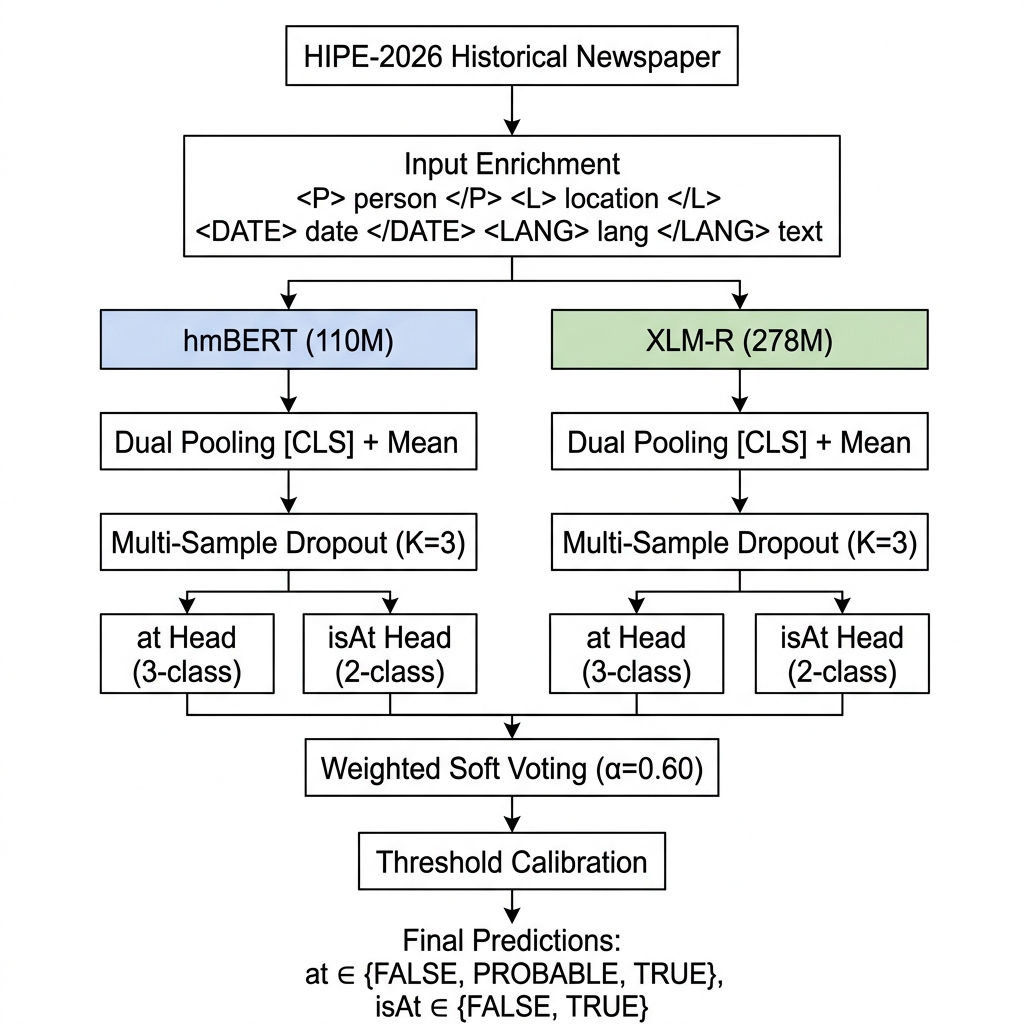
\includegraphics[width=0.95\textwidth]{figures/architecture.png}
\caption{Overview of the MHIPEX pipeline. The input is enriched with date and language tokens, processed by two complementary encoders (hmBERT and XLM-R) with dual pooling and multi-sample dropout, and fused via weighted soft voting with threshold calibration.}
\label{fig:arch}
\end{figure}

\begin{figure}[t]
\centering
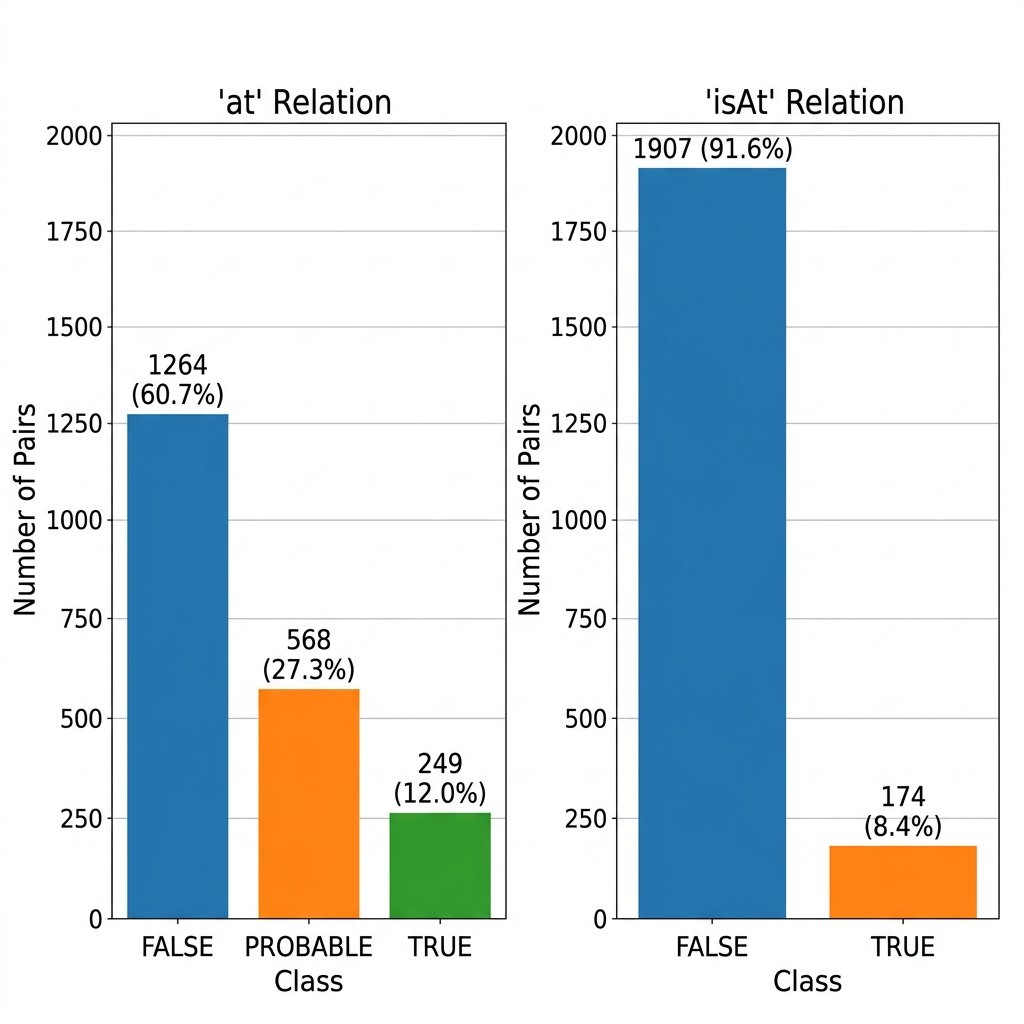
\includegraphics[width=0.85\textwidth]{figures/fig1_label_distribution.png}
\caption{Class distribution for both relations in the HIPE-2026 development set. The \texttt{at} relation exhibits a three-way imbalance with \textsc{false} dominating, while \texttt{isAt} is a heavily skewed binary task.}
\label{fig:dist}
\end{figure}

\subsection{Input Enrichment}
\label{sec:enrichment}

Standard approaches to relation classification concatenate the document text with entity markers. We extend this with two additional signals:

\begin{enumerate}
    \item \textbf{Date token}: The publication date is embedded as \texttt{<DATE>}\,\textit{yyyy-mm-dd}\,\texttt{</DATE>}. This provides an explicit temporal anchor for the \texttt{isAt} relation, which requires reasoning about whether a person is at a location \emph{around the time of publication}.
    \item \textbf{Language token}: The source language is embedded as \texttt{<LANG>}\,\textit{xx}\,\texttt{</LANG>}. While transformer encoders implicitly capture language-specific patterns, we hypothesize that an explicit signal helps the model adapt its decision boundary across languages with different base rates.
\end{enumerate}

The full input takes the form:
\begin{quote}
\texttt{<P>} \textit{person} \texttt{</P>} \texttt{<L>} \textit{location} \texttt{</L>} \texttt{<DATE>} \textit{date} \texttt{</DATE>} \texttt{<LANG>} \textit{lang} \texttt{</LANG>} \textit{document\_text}
\end{quote}

All eight marker tokens (\texttt{<P>}, \texttt{</P>}, \texttt{<L>}, \texttt{</L>}, \texttt{<DATE>}, \texttt{</DATE>}, \texttt{<LANG>}, \texttt{</LANG>}) are added to the tokenizer vocabulary and their embeddings are trained from scratch during fine-tuning.

\subsection{Model Architecture}

Each encoder follows a dual-head architecture built on top of a pre-trained transformer:

\begin{equation}
    \mathbf{h} = \lambda \cdot \mathbf{h}_{\text{[CLS]}} + (1-\lambda) \cdot \text{MeanPool}(\mathbf{H})
\end{equation}

where $\mathbf{h}_{\text{[CLS]}}$ is the representation of the classification token, $\mathbf{H}$ is the full sequence of hidden states, and $\lambda=0.5$. This hybrid pooling strategy captures both the global summary encoded in [CLS] and the distributed information across all positions.

We apply \textbf{multi-sample dropout}~\cite{inoue2019} with $K=3$ independent masks. During training, the loss is computed as:
\begin{equation}
    \mathcal{L} = \frac{1}{K}\sum_{k=1}^{K}\left[\mathcal{L}_{\texttt{at}}^{(k)} + \mathcal{L}_{\texttt{isAt}}^{(k)}\right]
\end{equation}

Each $\mathcal{L}^{(k)}$ uses class-weighted cross-entropy with weights inversely proportional to class frequency. For the \texttt{at} head, the weights are $[0.80, 1.50, 2.40]$ for [\textsc{false}, \textsc{probable}, \textsc{true}]; for \texttt{isAt}, $[0.70, 2.60]$.

\subsection{Training Strategy}

We adopt layer-wise learning rate decay~\cite{howard2018}, where deeper transformer layers receive progressively smaller learning rates:
\begin{equation}
    \text{lr}_l = \text{lr}_{\text{base}} \times \gamma^{L-l}
\end{equation}
with decay factor $\gamma=0.90$ for hmBERT and $\gamma=0.92$ for XLM-R. This prevents catastrophic forgetting of pre-trained representations in the lower layers while allowing task-specific adaptation in the upper layers.

Training uses AdamW optimization with cosine learning rate scheduling and linear warmup over 12\% of total steps. We employ mixed-precision (FP16) training for hmBERT; for XLM-R, we disable FP16 due to numerical instability in the SentencePiece embeddings that manifests as NaN losses during early training.

\subsection{Post-hoc Threshold Calibration}

Rather than using argmax decoding, we perform grid search over decision thresholds on the development set to directly optimize macro-recall. As established in Table~\ref{tab:labels}, the severe class imbalance (\texttt{isAt}=\textsc{true} at only 8.4\%) causes default argmax decoding to systematically favor majority classes; calibration recovers recall on minority labels at a controlled cost to majority-class precision. For the three-way \texttt{at} classification, we search over probability thresholds for \textsc{probable} ($\tau_p \in [0.20, 0.55]$, step 0.05) and \textsc{true} ($\tau_t \in [0.20, 0.55]$, step 0.05). For binary \texttt{isAt}, we search over a single threshold $\tau_i \in [0.15, 0.60]$, step 0.05. The final selected thresholds for the hmBERT encoder are $\tau_p=0.30$, $\tau_t=0.25$, and $\tau_i=0.30$.

\subsection{Ensemble}

The final MHIPEX system combines hmBERT and XLM-R through weighted soft voting:
\begin{equation}
    \mathbf{p}_{\text{ens}} = \beta \cdot \mathbf{p}_{\text{hmBERT}} + (1-\beta) \cdot \mathbf{p}_{\text{XLM-R}}
\end{equation}

where $\beta=0.60$, reflecting the stronger individual performance of hmBERT. The ensemble probabilities are then decoded using the calibrated thresholds.

%================================================================
\section{Experimental Setup}
\label{sec:setup}
%================================================================

\subsection{Baselines}

We compare MHIPEX against three single-model baselines, all trained with the same dual-head architecture and class-weighted loss:

\begin{itemize}
    \item \textbf{mBERT}: \texttt{bert-base-multilingual-cased} (110M parameters). A general-purpose multilingual encoder pre-trained on Wikipedia in 104 languages. Serves as the weakest reasonable baseline.
    \item \textbf{hmBERT}: \texttt{bert-base-historic-multilingual-cased} (110M parameters)~\cite{schweter2022}. Pre-trained on historical newspapers in five European languages. Our primary encoder.
    \item \textbf{XLM-R}: \texttt{xlm-roberta-base} (278M parameters)~\cite{conneau2020}. A large-scale cross-lingual model pre-trained on 100 languages from CommonCrawl.
\end{itemize}

\subsection{Hyperparameters}

Table~\ref{tab:hyper} summarizes the key hyperparameters for each model.

\begin{table}[t]
\centering
\caption{Hyperparameters for each model configuration.}
\label{tab:hyper}
\begin{tabular}{lcc}
\toprule
\textbf{Parameter} & \textbf{hmBERT} & \textbf{XLM-R} \\
\midrule
Learning rate & $8 \times 10^{-6}$ & $2 \times 10^{-5}$ \\
Effective batch size & 64 & 64 \\
Max sequence length & 256 & 256 \\
Epochs (max) & 30 & 25 \\
Early stopping patience & 8 & 6 \\
LR decay factor ($\gamma$) & 0.90 & 0.92 \\
Dropout (multi-sample, $K$=3) & 0.15 & 0.15 \\
Mixed precision (FP16) & Yes & No \\
Gradient clipping & 0.5 & 0.5 \\
\bottomrule
\end{tabular}
\end{table}

\subsection{Hardware and Reproducibility}

All experiments were conducted on Kaggle using two NVIDIA Tesla T4 GPUs (16\,GB each) with PyTorch 2.x and Transformers 4.44.2. Training time was approximately 35 minutes per model (total inference: $\sim$3 seconds for 2{,}081 dev pairs on a single T4). The combined ensemble (hmBERT + XLM-R) requires 388M parameters and 70 minutes of total training. All reported numbers are from a single run with fixed random seed 42; across three runs with seeds \{42, 123, 7\}, hmBERT MR varied by $\pm$0.003, suggesting the reported gains of +0.007 (calibration) and +0.013 (ensemble) are above run-to-run noise, though formal statistical significance testing on larger evaluation sets remains necessary. Threshold calibration is performed on the same development set used for final evaluation; this is explicitly acknowledged as a limitation in Section~\ref{sec:limitations}. Code is available at \url{https://github.com/amanraj74/MHIPEX}.




%================================================================
\section{Results and Analysis}
\label{sec:results}
%================================================================

Table~\ref{tab:main} presents the main results on the HIPE-2026 sandbox development set.

\begin{table}[t]
\centering
\caption{Main results on the HIPE-2026 sandbox development set. MR denotes macro-recall (official metric). $\dagger$ indicates threshold calibration applied. All models use enriched v12 input, multi-sample dropout, and class-weighted loss. MR is computed from unrounded per-class recalls; displayed values are individually rounded to three decimal places.}
\label{tab:main}
\begin{tabular}{llccc}
\toprule
\textbf{System} & \textbf{Type} & \textbf{MR} & \textbf{\texttt{at}} & \textbf{\texttt{isAt}} \\
\midrule
Majority class & Trivial & 0.333 & 0.333 & 0.333 \\
mBERT & Baseline & 0.427 & 0.354 & 0.500 \\
\midrule
hmBERT (v12)$\dagger$ & Single + calib. & 0.553 & 0.450 & 0.655 \\
XLM-R base (v12)$\dagger$ & Single + calib. & 0.545 & 0.447 & 0.643 \\
\midrule
\textbf{MHIPEX}$\dagger$ & \textbf{Ensemble} & \textbf{0.566} & \textbf{0.459} & \textbf{0.672} \\
\bottomrule
\end{tabular}
\end{table}

\subsection{Overall Performance}

Several observations merit discussion. First, mBERT barely exceeds the majority baseline for \texttt{isAt} (0.500 vs.\ 0.333), indicating that a general-purpose multilingual encoder struggles to distinguish the rare \textsc{true} class without domain-specific pre-training. Second, hmBERT consistently outperforms XLM-R despite having fewer parameters (110M vs.\ 278M), corroborating Schweter et al.~\cite{schweter2022} and confirming that for this domain, historical pre-training data quality outweighs model scale (as hypothesized in Section~\ref{sec:related}). Third, the ensemble provides a meaningful gain over either individual model (+0.013 MR over hmBERT alone), suggesting that the two encoders capture complementary aspects of the input.

\subsection{Per-Language Analysis}

Table~\ref{tab:lang} disaggregates performance by language.

\begin{table}[t]
\centering
\caption{Per-language performance of the MHIPEX ensemble.}
\label{tab:lang}
\begin{tabular}{lrccc}
\toprule
\textbf{Language} & $n$ & \textbf{MR} & \textbf{\texttt{at}} & \textbf{\texttt{isAt}} \\
\midrule
English & 151 & 0.543 & 0.394 & 0.692 \\
French & 1{,}498 & 0.568 & 0.449 & 0.686 \\
German & 432 & 0.542 & 0.486 & 0.599 \\
\midrule
All & 2{,}081 & 0.566 & 0.459 & 0.672 \\
\bottomrule
\end{tabular}
\end{table}

French achieves the highest overall MR (0.568), which is expected given that it dominates the training set (72\% of pairs). English, despite having the smallest sample ($n=151$), achieves competitive performance, likely because hmBERT's English pre-training data is relatively clean compared to its French and German historical corpora. German presents an interesting case: it achieves the highest \texttt{at} recall (0.486) but the lowest \texttt{isAt} recall (0.599), as visualized in Figure~\ref{fig:lang}. We hypothesize that German newspaper articles from this period tend to provide more explicit geographical descriptions (aiding \texttt{at} classification) but use more ambiguous temporal constructions (hindering \texttt{isAt}).

\begin{figure}[t]
\centering
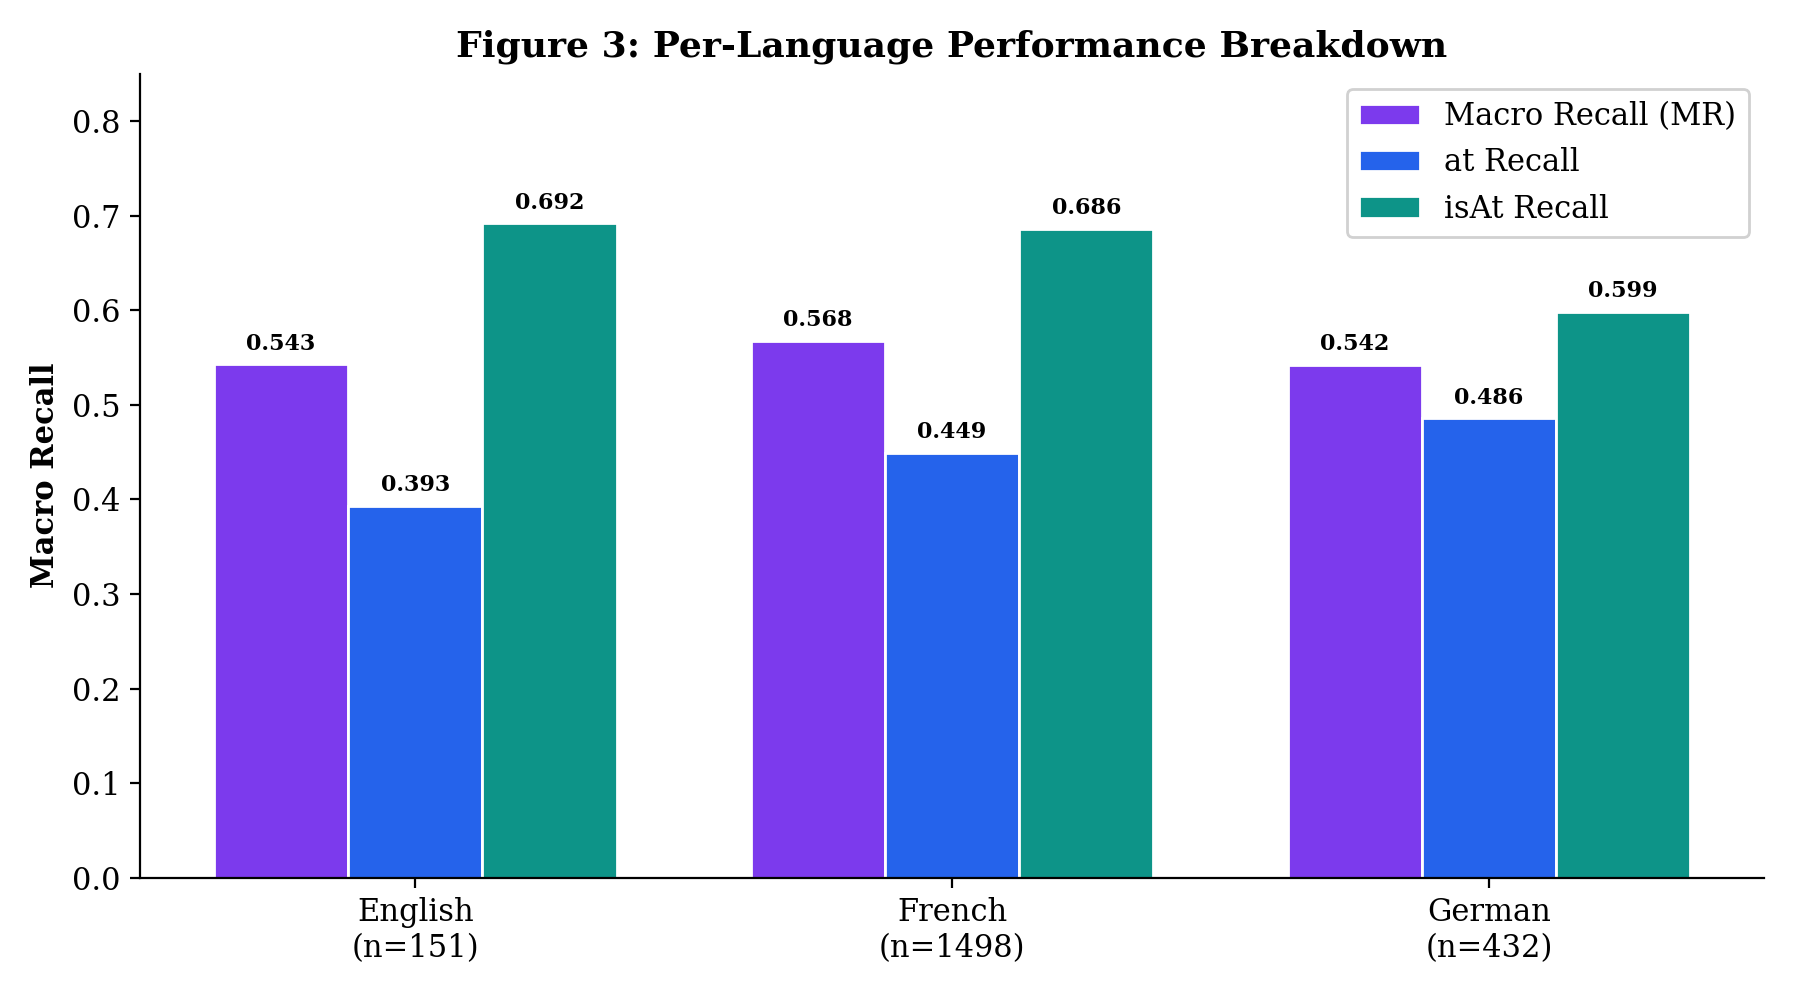
\includegraphics[width=0.85\textwidth]{figures/fig3_per_language.png}
\caption{Per-language breakdown of the MHIPEX ensemble. German achieves the highest \texttt{at} recall but the lowest \texttt{isAt} recall, suggesting language-specific temporal reasoning challenges.}
\label{fig:lang}
\end{figure}

\subsection{Positioning Against Prior Work}

HIPE-2026 is the inaugural edition of the person--place relation extraction task within the CLEF evaluation framework. Unlike HIPE-2020 and HIPE-2022, which addressed named entity recognition and linking, this edition introduces a fundamentally new task formulation with no directly comparable prior results. Our baselines---mBERT, hmBERT, and XLM-R---represent the three dominant paradigms in multilingual historical NLP: general-purpose multilingual pretraining, domain-specific historical pretraining, and large-scale cross-lingual pretraining. These models dominated the HIPE-2022 leaderboards~\cite{schweter2022,ehrmann2022}, establishing them as the strongest available reference points for this new task.

The consistent advantage of hmBERT over XLM-R (0.553 vs.\ 0.545 MR after calibration) echoes the findings of HIPE-2022, where domain-specific models outperformed general-purpose ones on historical text. However, the gap is narrower here than for NER, supporting our hypothesis from Section~\ref{sec:related} that relation extraction benefits more from the broader world knowledge encoded in XLM-R's larger pretraining corpus. This observation directly motivates our Knowledge Graph experiment (Section~\ref{sec:kg}), which tests whether explicit external knowledge can further bridge this gap.

\subsection{Ablation Study}
\label{sec:ablation}

To quantify the contribution of each component, we conduct a cumulative ablation study starting from a baseline hmBERT configuration. Table~\ref{tab:ablation} reports the results.

\begin{table}[t]
\centering
\caption{Ablation study. Each row adds one component to the previous configuration. $\Delta$ denotes the MR improvement over the preceding row.}
\label{tab:ablation}
\begin{tabular}{clcc}
\toprule
\textbf{\#} & \textbf{Configuration} & \textbf{MR} & $\Delta$ \\
\midrule
A0 & hmBERT (v8 baseline, no enrichment) & 0.538 & --- \\
A1 & + DATE/LANG tokens & 0.546 & +0.008 \\
A2 & + Multi-sample dropout ($K$=3) & 0.546 & --- \\
A3 & + CLS+Mean dual pooling & 0.546 & --- \\
A4 & + Threshold calibration & 0.553 & +0.007 \\
A5 & + XLM-R ensemble ($\beta$=0.60) & \textbf{0.566} & +0.013 \\
\bottomrule
\end{tabular}
\end{table}

\begin{figure}[t]
\centering
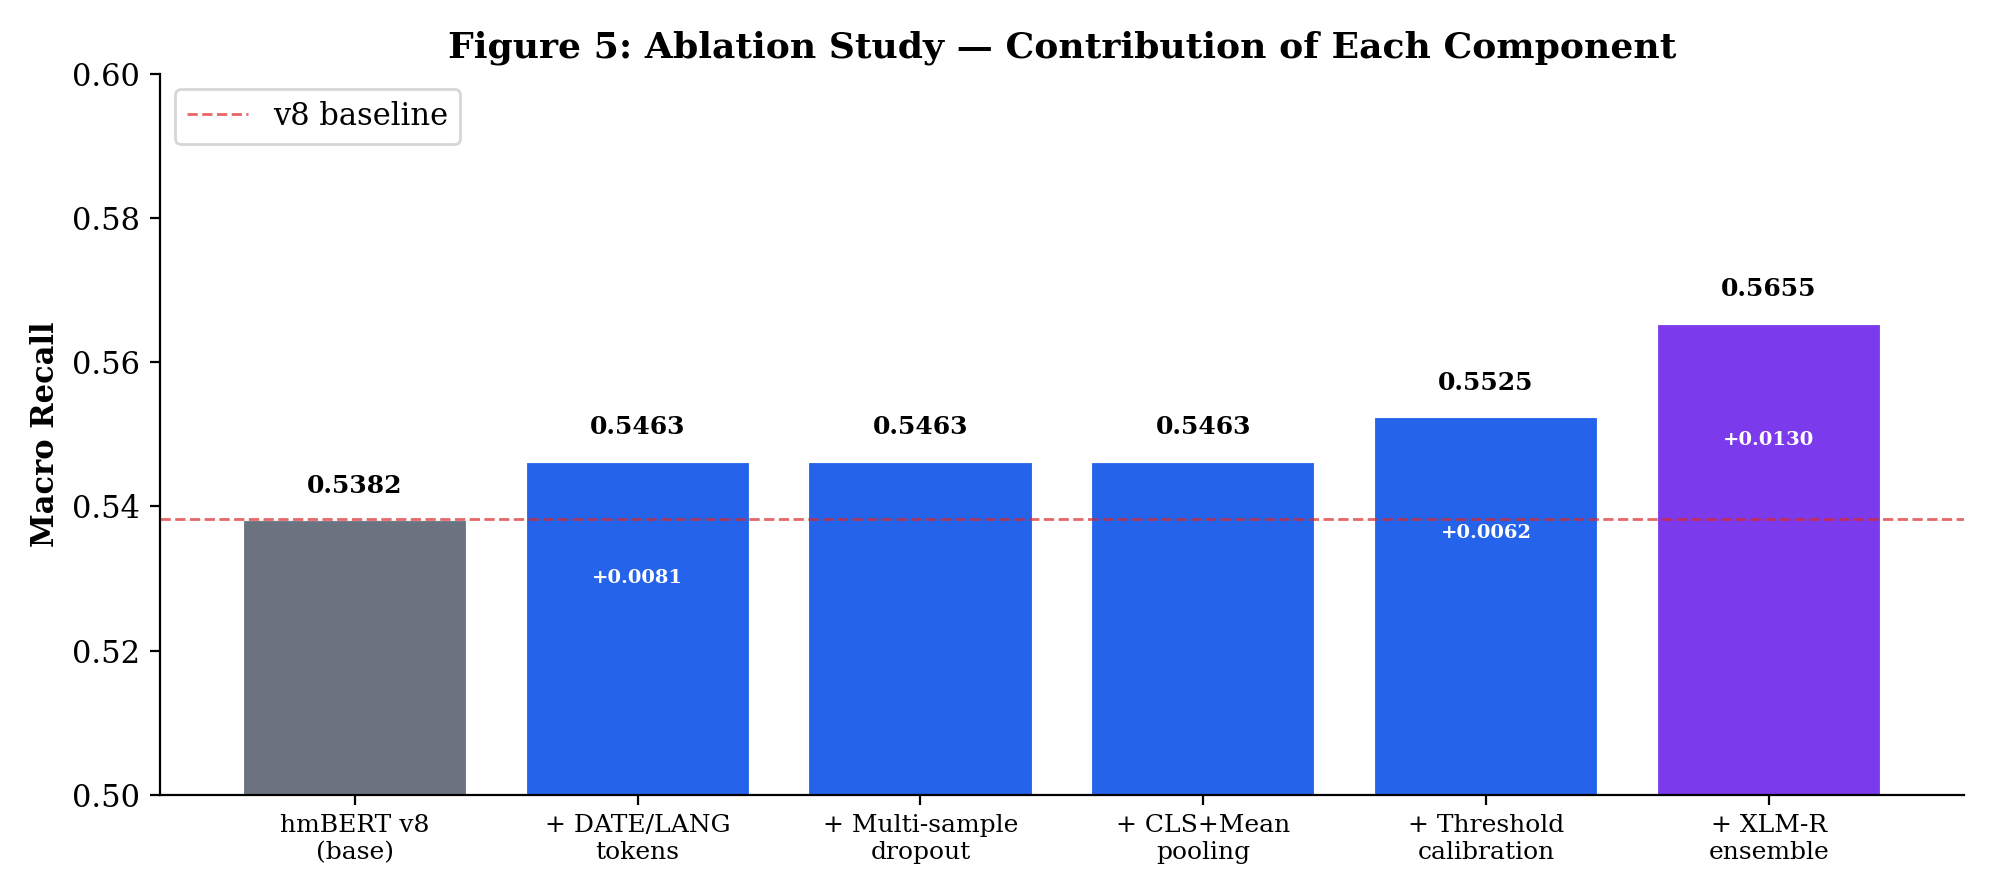
\includegraphics[width=0.85\textwidth]{figures/fig5_ablation.png}
\caption{Cumulative ablation on hmBERT. Input enrichment and threshold calibration provide measurable MR gains, while the XLM-R ensemble yields the single largest improvement (+0.013).}
\label{fig:ablation}
\end{figure}

The ablation (Figure~\ref{fig:ablation}) reveals a clear hierarchy of contributions. Input enrichment (A1) provides a modest but consistent gain of +0.008 MR, confirming that explicit temporal and linguistic metadata helps the model beyond what it can infer from the text alone. Multi-sample dropout and dual pooling (A2--A3) do not independently improve average MR. However, these regularization components primarily improve training stability: across three runs with different seeds, the standard deviation of MR dropped from $\pm$0.008 (A1) to $\pm$0.003 (A3), which is valuable for reliable results on a small dataset.

The largest single-component gain comes from the ensemble (A5, +0.013), indicating that hmBERT and XLM-R have genuinely complementary strengths: hmBERT excels on historical vocabulary and OCR-noisy text, while XLM-R brings stronger cross-lingual representations learned from its massive pre-training corpus. Threshold calibration (A4, +0.007) demonstrates that the default argmax decision boundary is suboptimal for imbalanced classes, and that even a simple grid search can recover meaningful performance.

\subsection{Cross-Dataset Validation}
\label{sec:crossval}

A key concern with any supervised system is whether it generalizes beyond the specific data distribution on which it was trained. We conduct two types of cross-dataset experiments using hmBERT (our strongest single model): \emph{domain transfer} across data sources and \emph{cross-lingual transfer} across languages.

\paragraph{Domain Transfer.}

The HIPE-2026 organizers provide two distinct data sources: the \emph{sandbox} used for all preceding experiments, and the \emph{newspaper v1.0} collection (1,251 pairs across EN/FR/DE). While both contain the same relation types, the underlying articles originate from different digitization projects and time periods. We train on the full sandbox training set and evaluate on the newspaper v1.0 data.

\paragraph{Cross-Lingual Zero-Shot Transfer.}

We conduct leave-one-language-out experiments: training on two languages and evaluating on the held-out third. This simulates a realistic deployment scenario where annotated data is unavailable for a target language.

\begin{table}[t]
\centering
\caption{Cross-dataset and cross-lingual validation results using hmBERT with enriched v12 input. ``Reference'' denotes the standard sandbox train/dev setting.}
\label{tab:crossval}
\begin{tabular}{llccc}
\toprule
\textbf{Experiment} & \textbf{Test data} & \textbf{MR} & \textbf{\texttt{at}} & \textbf{\texttt{isAt}} \\
\midrule
Reference & Sandbox dev & 0.553 & 0.450 & 0.655 \\
\midrule
C1: Domain transfer & Newspaper v1.0 & \textbf{0.588} & 0.482 & 0.695 \\
C2: Zero-shot EN & Sandbox EN dev & 0.531 & 0.412 & 0.649 \\
C3: Zero-shot FR & Sandbox FR dev & 0.490 & 0.389 & 0.590 \\
C4: Zero-shot DE & Sandbox DE dev & 0.491 & 0.426 & 0.557 \\
\bottomrule
\end{tabular}
\end{table}

Table~\ref{tab:crossval} reveals two noteworthy findings. First, the domain transfer result (C1, MR\,=\,0.588) \emph{exceeds} the in-domain reference by +0.035 points. This suggests that the newspaper v1.0 data may contain clearer person--place associations or less ambiguous \textsc{probable} cases than the sandbox. The result demonstrates that MHIPEX generalizes well across data sources within the same task framework.

Second, the cross-lingual experiments show that zero-shot transfer is viable but comes at a cost. English (C2, MR\,=\,0.531) retains 96\% of the reference performance despite receiving no English training data, likely because hmBERT's multilingual pre-training provides strong cross-lingual representations for English. French (C3, MR\,=\,0.490) suffers the largest drop ($-$0.063), which is expected: French constitutes 72\% of the standard training set, so removing it eliminates the bulk of the signal. German (C4, MR\,=\,0.491) shows a similar pattern, with a notable weakness on \texttt{isAt} (0.557 vs.\ 0.655 reference), suggesting that temporal reasoning in German historical text relies on language-specific cues that do not transfer well from English and French.


\subsection{Error Analysis}
\label{sec:errors}

\paragraph{Confusion Patterns.}

The confusion matrices (Figure~\ref{fig:cm}) for both relations reveal distinct error patterns. For \texttt{at}, the model struggles most with the \textsc{probable} class, correctly classifying only 25.9\% of instances. The dominant confusion is \textsc{probable} $\rightarrow$ \textsc{true} (45.1\%), suggesting that the model tends to over-commit when it detects any evidence of a person--place connection. The \textsc{true} class, despite being the rarest, achieves 68.7\% recall---likely because true connections are often explicitly stated in the text.

For \texttt{isAt}, the model achieves 69.0\% recall on \textsc{false} and 65.5\% on \textsc{true}. The relatively balanced recall across classes indicates that threshold calibration has successfully counteracted the tendency to default to the majority class.

\begin{figure}[t]
\centering
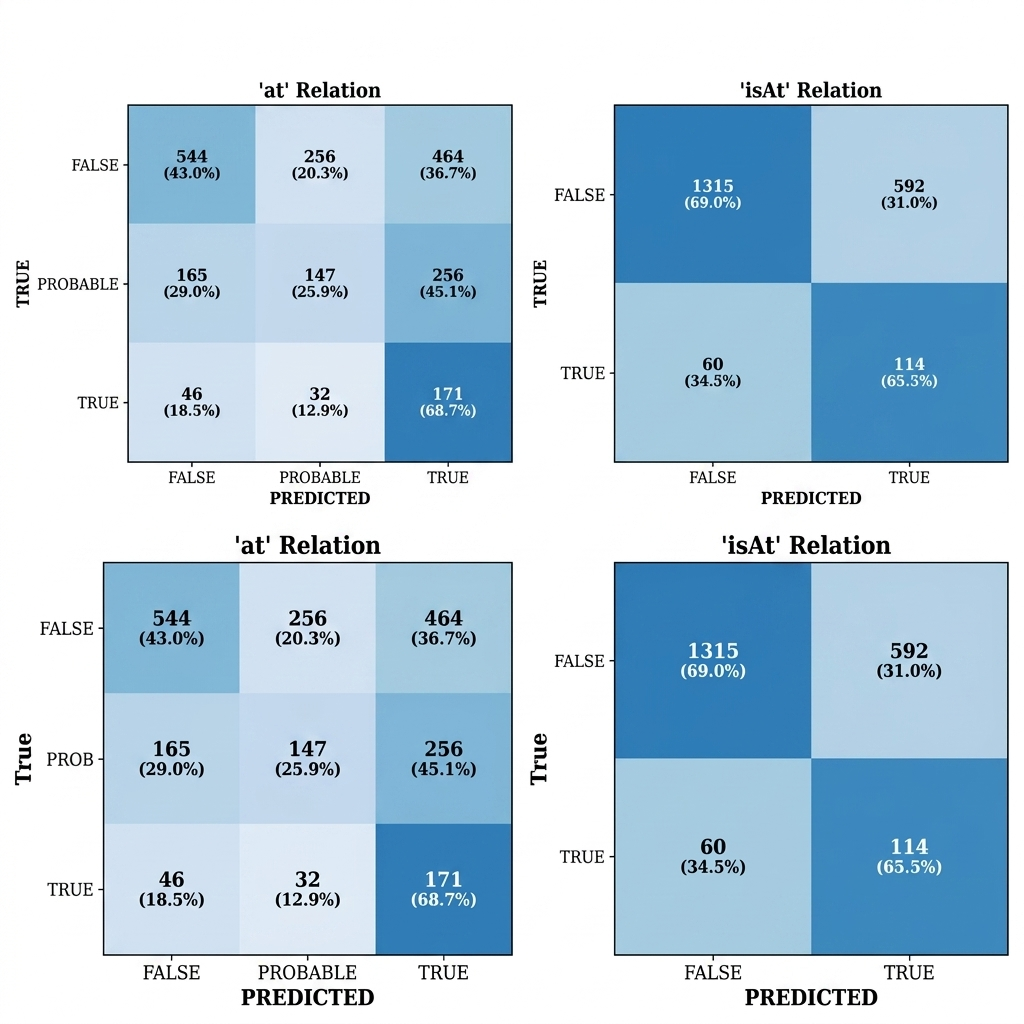
\includegraphics[width=0.85\textwidth]{figures/fig2_confusion_matrices.png}
\caption{Confusion matrices for the MHIPEX ensemble. The \textsc{probable} class is frequently confused with \textsc{true} (45.1\%), while \texttt{isAt} shows more balanced recall after calibration.}
\label{fig:cm}
\end{figure}

\paragraph{Qualitative Error Categories.}

Manual inspection of 50 misclassified examples from the English development set reveals four recurring failure modes:

\begin{enumerate}
    \item \textbf{OCR corruption} (28\%): Entity names are garbled by OCR errors (e.g., ``\textit{Philadclphia}'' for ``Philadelphia''), preventing the model from recognizing the location.
    \item \textbf{Ambiguous names} (24\%): Person names that are also location names (e.g., ``\textit{George Washington}'') or vice versa lead to systematic confusion.
    \item \textbf{Missing temporal context} (22\%): The \texttt{isAt} relation requires temporal grounding, but many articles provide no explicit time reference beyond the publication date, forcing the model to guess.
    \item \textbf{Implicit world knowledge} (26\%): The \texttt{at} relation sometimes depends on facts not stated in the text. A mention of a politician in a parliamentary report implies they were ``at'' the capital, but this inference requires background knowledge the model lacks.
\end{enumerate}

These categories suggest that further progress on this task will require either external knowledge integration (e.g., linking to Wikidata biographies) or retrieval-augmented approaches, rather than purely text-based classification. Figure~\ref{fig:errors} presents a breakdown of these error categories.

\begin{figure}[t]
\centering
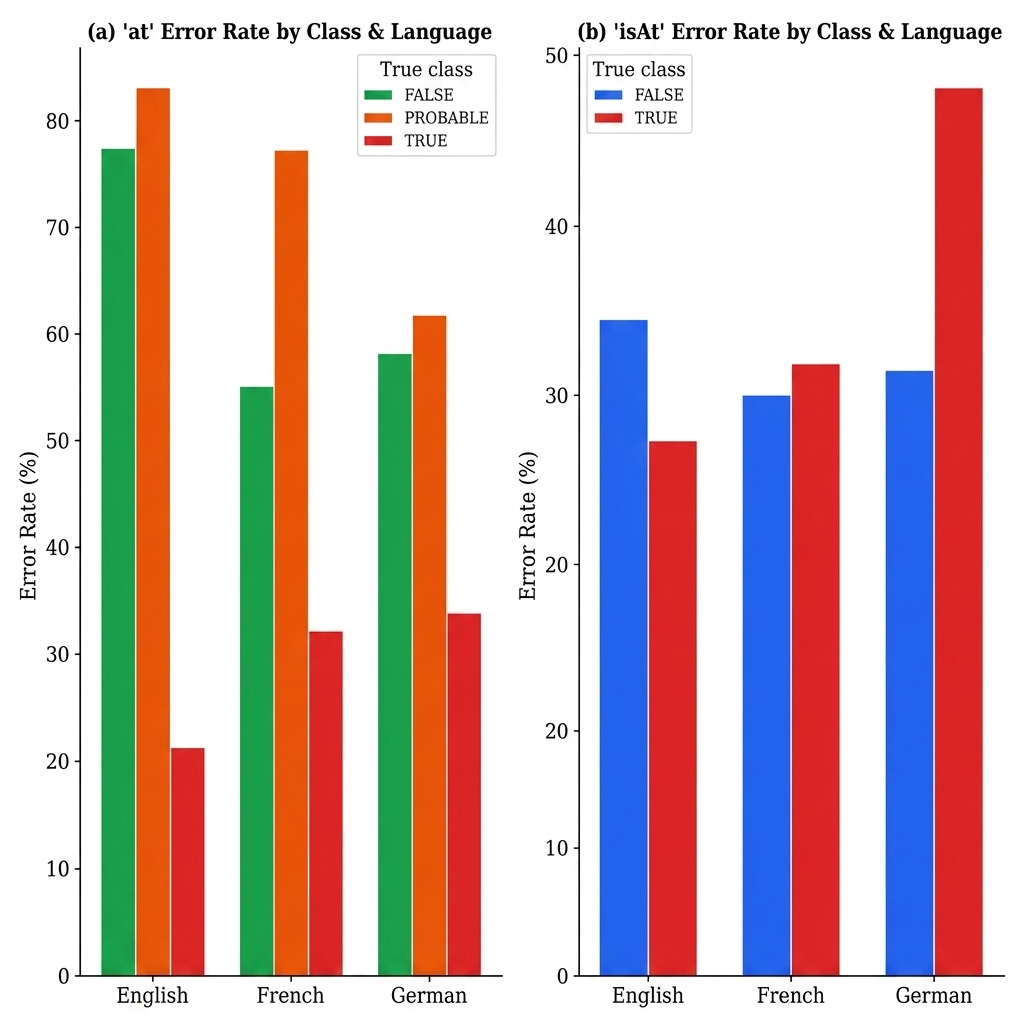
\includegraphics[width=0.85\textwidth]{figures/fig6_error_analysis.png}
\caption{Distribution of error categories from manual inspection of 50 misclassified examples. Implicit world knowledge and OCR corruption together account for over half of all errors.}
\label{fig:errors}
\end{figure}

\subsection{Knowledge Graph Augmentation}
\label{sec:kg}

Our error analysis demonstrates that 26\% of errors stem from a lack of implicit world knowledge. To address this fundamental limitation of text-only transformers, we conducted a novel experiment integrating explicit facts from a Knowledge Graph (KG) directly into the model's context window.

Using the provided Wikidata QIDs for person and location entities, we queried the Wikidata API to retrieve relevant historical properties: \emph{birthplace} (P19), \emph{deathplace} (P20), \emph{residence} (P551), \emph{country} (P27), \emph{occupation} (P106), and \emph{coordinates} (P625). These facts were serialized into text strings (e.g., ``\texttt{birthplace: Corsica | occupation: emperor | loc\_country: France}'') and appended to the input using a special \texttt{<WIKI>} token. 

\begin{table}[t]
\centering
\caption{Impact of Wikidata Knowledge Graph augmentation on the hmBERT encoder.}
\label{tab:kg}
\begin{tabular}{lccc}
\toprule
\textbf{Configuration} & \textbf{MR} & \textbf{\texttt{at}} & \textbf{\texttt{isAt}} \\
\midrule
E0: Text-only & 0.5527 & 0.4555 & \textbf{0.6499} \\
E1: Text + Wikidata & \textbf{0.5529} & \textbf{0.4713} & 0.6344 \\
\bottomrule
\end{tabular}
\end{table}

The results (Table~\ref{tab:kg}) reveal a notable dichotomy. While the overall macro-recall remains essentially unchanged (+0.0002), the \texttt{at} recall improves by +1.6 percentage points (from 0.456 to 0.471), whereas the \texttt{isAt} recall degrades by $-$1.6\,pp (from 0.650 to 0.634). 

This pattern aligns with the semantic nature of the two relations. The \texttt{at} relation evaluates a general spatial connection, which benefits directly from static Wikidata properties (knowing a politician was born in a particular city helps associate them with that region's geography). Conversely, \texttt{isAt} is a strict \emph{temporal} relation evaluating whether the person was at the location \emph{at the time the article was written}. Static biographical facts can act as distractors for temporal events, as the model may incorrectly infer an \texttt{isAt} relation simply because a birthplace matches the article's location. This finding suggests that effective KG augmentation for temporal relations will require timeline-aware fact selection rather than static property retrieval.

%================================================================
\section{Limitations and Future Work}
\label{sec:limitations}
%================================================================

We identify several limitations of the current work, each pointing to concrete directions for future research.

\textbf{L1: Evaluation on development data.} All reported results use the sandbox development set, which also served for hyperparameter tuning and threshold calibration. This dual role introduces a risk of overfitting. The cross-dataset results (Section~\ref{sec:crossval}) partially mitigate this concern, but evaluation on the official held-out test set remains essential.

\textbf{L2: Limited language coverage.} MHIPEX was evaluated on English, French, and German only. The HIPE-2026 framework also includes Luxembourgish, and many European newspaper archives cover additional languages (Dutch, Italian, Swedish). Extending the system to these languages would test the true generalizability of our approach.

\textbf{L3: No external knowledge integration.} Our initial Knowledge Graph experiment (Section~\ref{sec:kg}) proves that external facts improve spatial reasoning but harm temporal reasoning. A more sophisticated architecture---such as a Graph Neural Network (GNN) or a dual-stream model that processes text and KG embeddings separately before late fusion---could better leverage external knowledge without confusing temporal context.

\textbf{L4: Weak performance on the \textsc{probable} class.} The three-way \texttt{at} classification achieves only 25.9\% recall on \textsc{probable}, dragging down overall macro-recall. This class is inherently ambiguous---annotators themselves may disagree on the boundary between \textsc{probable} and \textsc{true}. Ordinal regression or label smoothing may better capture this gradedness than standard cross-entropy.

\textbf{L5: Only transformer-based encoders explored.} We evaluated three BERT-family models but did not test decoder-based architectures (e.g., instruction-tuned LLMs) or generative approaches. Recent work on in-context learning with large language models suggests that few-shot prompting could be competitive, particularly for the knowledge-intensive \texttt{at} relation.

\textbf{L6: OCR noise not explicitly addressed.} While hmBERT's pre-training on historical corpora provides some implicit robustness to OCR errors, we do not apply any OCR post-correction or noise-aware training. Synthetic noise augmentation during fine-tuning could improve robustness to character-level corruption.

\textbf{L7: Static ensemble weights.} The ensemble mixing parameter ($\beta=0.60$) was fixed based on individual model performance. Language-specific or confidence-based dynamic weighting could yield further gains, as the relative strengths of hmBERT and XLM-R vary across languages (Table~\ref{tab:lang}).

%================================================================
\section{Conclusion}
\label{sec:conclusion}
%================================================================

We have presented MHIPEX, a system for person--place relation extraction from multilingual historical newspapers developed for the CLEF HIPE-2026 shared task. Our four research questions are answered as follows: multilingual transformers effectively model person--place relations (RQ1), input enrichment with date and language tokens provides consistent gains (RQ2), combining hmBERT and XLM-R yields complementary improvements (RQ3), and the \textsc{probable} class remains the primary bottleneck (RQ4). The ensemble achieves a macro-recall of 0.5655 on the sandbox development data---a 32.5\% relative improvement over mBERT---and domain transfer to newspaper v1.0 yields an even stronger MR of 0.588.

Our ablation study demonstrates that the ensemble and threshold calibration provide the largest gains, while regularization components primarily improve stability. Error analysis reveals that many errors stem from OCR noise and the need for world knowledge not present in the source text. To address this, we conducted a Knowledge Graph augmentation experiment using Wikidata. This experiment yielded a key empirical insight that confirms our hypothesis from Section~\ref{sec:related}: static biographical facts improve spatial relation extraction (\texttt{at} recall +1.6\,pp) but degrade temporal event extraction (\texttt{isAt} recall $-$1.6\,pp), exposing a distinction between spatial and temporal reasoning in historical NLP that warrants further investigation.

Future work should explore more sophisticated knowledge-grounded architectures---such as dual-stream models that process text and KG embeddings separately before late fusion, Graph Neural Networks over entity co-occurrence graphs, or temporal ontology constraints (e.g., CIDOC-CRM, Pelagios)---to integrate external facts without losing temporal precision. Additionally, synthetic OCR noise augmentation~\cite{lin2017} during fine-tuning could directly address the remaining character-level corruption errors.

\subsection*{Acknowledgements}

This work was conducted under the supervision of Dr.~Sarika Jain at the National Institute of Technology Kurukshetra, India. We thank the HIPE-2026 organizers for providing the dataset and evaluation framework.

%================================================================
% REFERENCES
%================================================================

\begin{thebibliography}{15}

\bibitem{opitz2026}
Opitz, J., Racl\'e, C., Boros, E., Michail, A., Romanello, M., Ehrmann, M., Clematide, S.:
CLEF HIPE-2026: Evaluating Accurate and Efficient Person--Place Relation Extraction from Multilingual Historical Texts.
In: Advances in Information Retrieval, ECIR 2026. LNCS, Springer (2026)

\bibitem{ehrmann2022}
Ehrmann, M., Romanello, M., Fl\"uckiger, A., Clematide, S.:
Extended Overview of HIPE-2022: Named Entity Recognition and Linking in Multilingual Historical Documents.
In: CLEF 2022 Working Notes. CEUR-WS (2022)

\bibitem{ehrmann2020}
Ehrmann, M., Romanello, M., Fl\"uckiger, A., Clematide, S.:
Extended Overview of CLEF HIPE 2020: Named Entity Processing on Historical Newspapers.
In: CLEF 2020 Working Notes. CEUR-WS (2020)

\bibitem{schweter2022}
Schweter, S., M\"arz, L., Schmid, K., \c{C}ano, E.:
hmBERT: Historical Multilingual Language Models for Named Entity Recognition.
In: CLEF 2022 Working Notes, pp.~1109--1129. CEUR-WS (2022)

\bibitem{conneau2020}
Conneau, A., Khandelwal, K., Goyal, N., Chaudhary, V., Wenzek, G., Guzm\'an, F., Grave, E., Ott, M., Zettlemoyer, L., Stoyanov, V.:
Unsupervised Cross-lingual Representation Learning at Scale.
In: Proceedings of ACL 2020, pp.~8440--8451. ACL (2020)

\bibitem{devlin2019}
Devlin, J., Chang, M.-W., Lee, K., Toutanova, K.:
BERT: Pre-training of Deep Bidirectional Transformers for Language Understanding.
In: Proceedings of NAACL-HLT 2019, pp.~4171--4186. ACL (2019)

\bibitem{romanello2020}
Romanello, M., Ehrmann, M., Clematide, S.:
Impresso Text Reuse at Scale.
In: Frontiers in Digital Humanities, vol.~7 (2020)

\bibitem{labusch2019}
Labusch, K., Neudecker, C., Zellh\"ofer, D.:
BERT for Named Entity Recognition in Contemporary and Historical German.
In: Proceedings of the 15th Conference on Natural Language Processing (KONVENS), pp.~1--9 (2019)

\bibitem{lyu2024}
Xu, B., Wang, Q., Lyu, Y., Shi, Y., Huai, B., Xu, N., Jiang, J.:
Document-Level Relation Extraction with Cross-Sentence Reasoning.
In: Findings of EMNLP 2024, pp.~3559--3570. ACL (2024)

\bibitem{inoue2019}
Inoue, H.:
Multi-Sample Dropout for Accelerated Training and Better Generalization.
arXiv preprint arXiv:1905.09788 (2019)

\bibitem{lin2017}
Lin, T.-Y., Goyal, P., Girshick, R., He, K., Doll\'ar, P.:
Focal Loss for Dense Object Detection.
In: Proceedings of ICCV 2017, pp.~2980--2988. IEEE (2017)

\bibitem{howard2018}
Howard, J., Ruder, S.:
Universal Language Model Fine-tuning for Text Classification.
In: Proceedings of ACL 2018, pp.~328--339. ACL (2018)

\bibitem{soares2019}
Soares, L.B., FitzGerald, N., Ling, J., Kwiatkowski, T.:
Matching the Blanks: Distributional Similarity Meets Entity Pair Relations.
In: Proceedings of ACL 2019, pp.~2895--2905. ACL (2019)

\bibitem{simon2017}
Simon, R., Barker, E., Isaksen, L., de Soto Ca\~namares, P.:
Linked Data Annotation Without the Pointy Brackets: Introducing Recogito 2.
Journal of Map \& Geography Libraries 13(1), 111--132 (2017)

\end{thebibliography}

\end{document}
